%---------- Inleiding ---------------------------------------------------------

\section{Introductie} % The \section*{} command stops section numbering
\label{sec:introductie}

In 1991 werd Python voor het eerst gereleaset door Guido Van Rossum. Zijn visie over de scriptingtaal was duidelijk:
\begin{itemize}
	\item Gemakkelijk aan te leren
	\item Krachtig
	\item Open-source
\end{itemize}
Enkele jaren terug zien we dat Pyhon terug aan een sterke opmars bezig is. Dat komt door de komst van enkele nieuwe technologieën zoals: Machine Learning, Artificiële Intelligentie, Data mining, analyse van datagegevens, … Niet alleen wordt de scriptingtaal gebruikt voor nieuwere technologieën, maar ook bijvoorbeeld voor web development en hacking. Kortom, Python is terug hot.
 
Maar hoe zit het bij de kennis van Python bij de studenten die afgestudeerd zijn in de Toegepaste Informatica? Is deze voldoende om het werkveld te betreden? Of merken we dat werkgevers nog moeten investeren in hun om toch een degelijke kennis te vormen? 

Dit onderzoek zal uitwijzen of de kennisverwerving van Python wel degelijk een toegevoegde waarde is in de opleidingen Toegepaste Informatica. Dit zal gemeten worden aan de hand van wat er effectief gevraagd wordt in het werkveld.

%---------- Stand van zaken ---------------------------------------------------

\section{State-of-the-art}
\label{sec:state-of-the-art}

Een specifiek onderzoek naar hoe de kennis van Python is bij afgestudeerde studenten van de opleiding Toegepaste Informatica (in België) is tot op heden nog niet gebeurd. Wel zijn er talloze statistieken over de community rond Python (op populaire fora) en naar wat de vraag van uit het werkveld is naar de kennis hiervan.  

Wanneer we het artikel er bij nemen van \textcite{Cisco2018}, lezen we letterlijk: “Python is nog altijd een grote onbekende in bachelor- en masteropleidingen informatica. Hoewel inmiddels al bijna dertig jaar oud, is Python toch een van de programmeertalen van de toekomst.”. Cisco organiseerde daarom een eerste Python-challenge dit jaar in België. Hun doel is om de taal meer onder de aandacht te brengen. 

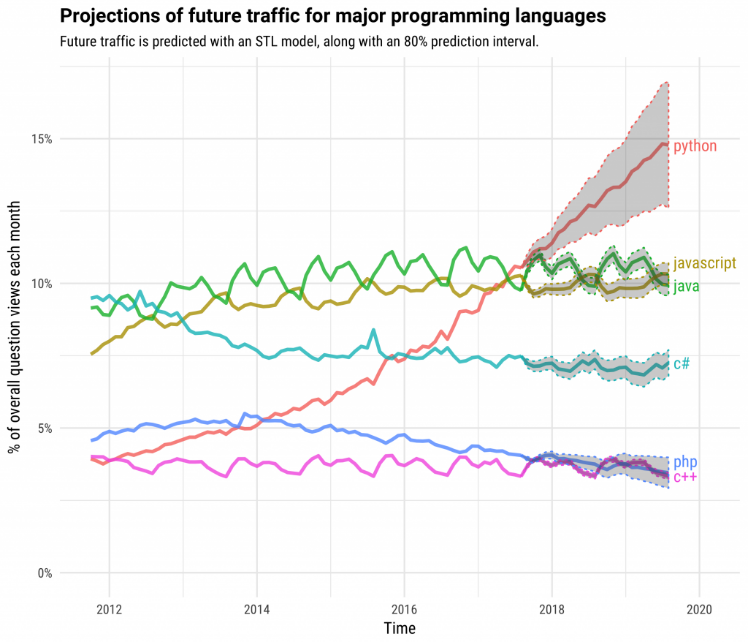
\includegraphics{graph.png}

Als we bovenstaande grafiek er bij nemen \autocite{SO2017}, zien we dat de groei van het aantal topics rond Python op Stackoverflow afgelopen jaren toeneemt. Op deze grafiek wordt ook een voorspelling gemaakt naar hoe dit zal zijn naar de toekomst. Hieruit kunnen we toch concluderen dat Python nog steeds een sterke groei zal hebben wat betreft het aantal gestelde vragen op het forum. Dit kan betekenen dat de populariteit van Python nog steeds exponentieel zal stijgen. 




% Voor literatuurverwijzingen zijn er twee belangrijke commando's:
% \autocite{KEY} => (Auteur, jaartal) Gebruik dit als de naam van de auteur
%   geen onderdeel is van de zin.
% \textcite{KEY} => Auteur (jaartal)  Gebruik dit als de auteursnaam wel een
%   functie heeft in de zin (bv. ``Uit onderzoek door Doll & Hill (1954) bleek
%   ...'')


%---------- Methodologie ------------------------------------------------------
\section{Methodologie}
\label{sec:methodologie}

Dit onderzoek zullen we op delen in een aantal delen. Het eerste deel omvat een onderzoek van het aanbod van de hogescholen. Krijgen de studenten wel degelijk Python in hun studies? Bekijken ze Python de algemene opleidingsonderdelen, of enkel in bepaalde specialisatierichtingen? Hoe uitgebreid zien deze studenten deze topic?

In het tweede deel van het onderzoek zullen we bekijken hoe de situatie is naar de vraag van de kennis en beheersing van Python. Zien we hier een significante stijging doorheen de jaren? Hoe zal dit zijn naar de toekomst toe? Daarnaast zullen er een aantal interviews afgenomen worden met werkgevers die op zoek zijn naar profielen met de kennis van Python. Enkele vragen die kunnen gesteld worden zijn: Zijn de juiste profielen makkelijk te vinden op de arbeidsmarkt? Hebben schoolverlaters een degelijke kennis van Python? Moet er nog veel geïnvesteerd worden in het opleiden van werknemers?

Het laatste deel van het onderzoek bestaat dan uit het bestuderen van de scriptingtaal zelf. Wat zijn nu de mogelijkheden met Python? Is deze taal makkelijk aan te leren? Wat brengt de toekomst? Is er een degelijke community opgebouwd rond Python?  Zijn IT’ers geïnteresseerd om deze taal aan te leren? Welke frameworks zijn er beschikbaar en wat zijn de mogelijkheden hiervan?


%---------- Verwachte resultaten ----------------------------------------------
\section{Verwachte resultaten}
\label{sec:verwachte_resultaten}

Op basis van het uitgevoerde onderzoek zullen we hiervan een resultaat kunnen opstellen. De resultaten die in verwacht zijn dat er niet genoeg tijd en middelen geïnvesteerd worden in het opbouwen van een goede kennis rond Python op de hogescholen als je dit vergelijkt met het aanbod van de werkelijke jobs op de arbeidsmarkt. Volgens mij moeten werkgevers wel nog degelijk schoolverlaters opleiden op gebied van hun Python kennis en dat de vraag naar ervaren programmeurs hierin groot is en zal blijven groeien.

%---------- Verwachte conclusies ----------------------------------------------
\section{Verwachte conclusies}
\label{sec:verwachte_conclusies}

Voor Hogescholen en Universiteiten zal het uiteraard een afweging zijn om Python uitgebreid aan te bieden in hun gamma. In de informatica heb je veel deeldomeinen en veel verschillende technologieën. Ik verwacht dat Python toch wel een aandeel zal hebben in veel van deze domeinen, en dus toch wel een enorme toegevoegde waarde kan zijn in de opleiding Toegepaste Informatica. Zowel bij programmeren, web development als bij netwerken kan Python gebruikt worden. Het is een zeer krachtige en eenvoudige taal, waarbij er heel wat mogelijk is. Het aanbod in het werkveld zal ook een grote rol spelen op de gemaakte conclusie.

